\documentclass[12pt]{report}
\usepackage[top=2.5cm, bottom=2.5cm, left=4cm, right=2.5cm, centering, head=21.75 pt]{geometry}

%\linespread{1.5}

\usepackage{amsmath}
\usepackage{amsthm}
\usepackage{subfigure}
\usepackage{booktabs}
\usepackage{caption}
\usepackage{amssymb}

\usepackage[italian]{babel}
\usepackage[utf8]{inputenc}
\usepackage{scrlayer-scrpage}
\ifoot[]{}
\cfoot[]{}
\ofoot[\pagemark]{\pagemark}
\pagestyle{scrplain}
\usepackage{mathptmx}
\usepackage{graphicx}
\usepackage{csquotes}
\usepackage[backend=biber, sorting=nty, ]{biblatex}
\appto{\bibsetup}{\raggedright}
\addbibresource{Thesis.bib}

\usepackage{titlesec}
\usepackage{float}

\usepackage{listings}
\renewcommand{\lstlistingname}{Code}
\usepackage{xcolor}
\definecolor{mygreen}{rgb}{0,0.6,0}
\definecolor{mygray}{rgb}{0.5,0.5,0.5}
\definecolor{mymauve}{rgb}{0.58,0,0.82}
\definecolor{darkgray}{rgb}{.4,.4,.4}
\definecolor{navy}{HTML}{000080}
\definecolor{purple}{rgb}{0.65, 0.12, 0.82}
\definecolor{codepurple}{rgb}{0.58,0,0.82}
\definecolor{backcolour}{rgb}{0.95,0.95,0.92}

\titleformat{\chapter}[block]
	{\normalfont\LARGE\bfseries}{\thechapter.}{0.5em}{\LARGE}
\titlespacing*{\chapter}{0pt}{-20pt}{25pt}

\usepackage{boxedminipage}
\usepackage{pgfplotstable}

\begin{document}

	\begin{titlepage}
		\begin{center}
			{\LARGE{Università degli Studi di Milano Bicocca \\}}
			{\small{Dipartimento di Informatica, Sistemistica e Comunicazione}}\\
			{\small{Corso di Laurea Triennale}}
		\end{center}
			
		\begin{figure}[H]
			\centering
			%\includegraphics[width=0.4\textwidth]{Logo.png}
		\end{figure}

		\begin{center}
			{\Large { ??? }}
		\end{center}

		\vspace{2cm}

		\begin{minipage}[t]{0.47\textwidth}
			{\large{\bf Relatore:\\ XXX YYY}}
			\vspace{0.5cm}
			{\large{\bf \\Correlatore:\\ XXX YYY}}
		\end{minipage}\hfill\begin{minipage}[t]{0.47\textwidth}\raggedleft
			{\large{\bf Candidato: \\XXX YYY\\ }}
		\end{minipage}

		\vspace{25mm}

		\centering{\large{\bf ANNO ACCADEMICO 2023/2024 }}
	\end{titlepage}

	\tableofcontents
	\thispagestyle{empty}

	\listoffigures
	\thispagestyle{empty}
	\clearpage

	\setcounter{page}{1}
	%\addtocontents{toc}{\protect\thispagestyle{empty}}
	%\addcontentsline{toc}{chapter}{Introduzione}
	%\input{introduzione.tex}

	%\clearpage

	%\input{capitolo1.tex}

	%\clearpage

	%\addcontentsline{toc}{chapter}{Conclusioni}
	%\input{conclusioni.tex}

	\chapter{Abstract}

		Silhouette é una metrica spesso utilizzata per individuare
		la combinazione di iperparametri di un algoritmo di clustering
		non supervisionato che risulti nel clustering piú vicino possibile
		alla vera struttura di cluster dei dati in analisi. Verrá introdotta
		Silhouette e come calcolarla, alcune proprietá matematiche ed alcune
		applicazioni concrete su dataset di EHR (\textit{Electronic Health
		Records}). Verranno inoltre analizzati alcuni pacchetti per il
		linguaggio \texttt{R} che implementano Silhouette per determinare
		quale sia il migliore, comparandone le performance sia fra di
		loro sia rispetto all'implementazione di \texttt{scikit-learn}
		(\texttt{Python}).

	\chapter{Clustering}

		Clustering è suddividere un dataset di un certo numero di elementi
		in sottoparti chiamate cluster sulla base della loro affinità.

		Il problema è che diversi algoritmi di clustering non sono in grado di
		fornire una metrica oggettiva per determinare quanto il clustering che
		hanno indotto sia effettivamente rappresentativo della struttura del
		dataset, o se sia semplicemente un raggruppamento arbitrario. Inoltre,
		diversi algoritmi come K-Means richiedono il numero di cluster come
		iperparametro, rendendo il discorso ancora più complesso, perché in
		genere nel clustering non supervisionato non vi è a disposizione
		alcuna "ground truth".

		La metrica Silhouette, introdotta per la prima volta in \cite{ROUSSEEUW198753},
		si propone di rispondere alle seguenti domande:

		\begin{itemize}
			\item
			Il clustering è di buona qualità? In altre parole, gli elementi di
			uno stesso cluster sono fra di loro "vicini" ed al contempo "lontani"
			dagli elementi di tutti gli altri cluster?
			\item
			Quali sono gli elementi ben classificati, ovvero quelli che probabilmente
			si trovano nel cluster "giusto"?
			\item
			Quali sono gli elementi che è difficile stabilire con certezza in quali
			cluster vadano collocati, ovvero quelli che stanno "nel mezzo" fra più
			cluster?
			\item
			Il numero di cluster scelto è effettivamente rappresentativo del dataset
			o è 'artificioso'?
		\end{itemize}

	\chapter{Silhouette}

		\section{Setup}

			Si supponga di avere a disposizione un dataset di dimensione
			$N \times M$, dove $N$ indica il numero degli elementi e $M$ è
			il numero di attributi. Per comodità, si assuma che gli attributi
			siano tutti dati numerici (altezze, lunghezze, capacità, ecc...).
			Per ogni elemento, tutti i valori di ciascun attributo sono noti.

			A partire da tale dataset è possibile costruire quella che viene
			chiamata \textbf{matrice delle distanze}. Tale matrice ha dimensione
			$N \times N$ e, in ciascuna cella $(i, j)$, è presente un valore
			indicato con $d(i, j)$ che rappresenta il grado di "dissomiglianza"
			fra l'elemento $i$ e l'elemento $j$ del dataset.

			Tale grado di dissomiglianza è calcolato mediante una
			\textbf{funzione di distanza}, usando come input i valori
			degli attributi di $i$ e di $j$. Un esempio di funzione di
			distanza è la \textbf{distanza Euclidea}, definita come segue:

			\begin{equation}
				d(i, j) =
				\sqrt{\sum_{m = 1}^{M} (f_{i, m} - f_{j, m})^{2}} =
				\sqrt{(f_{i, 1} - f_{j, 1})^{2} + \dots +
					(f_{i, M} - f_{j, M})^{2}}
			\end{equation}

			Dove $f_{i, m}$ e $f_{j, m}$ indicano il valore del $m$-esimo
			attributo per, rispettivamente, l'$i$-esimo ed il $j$-esimo
			elemento del dataset.

			Altri esempi di distanze sono la \textbf{distanza di Manhattan}
			e la \textbf{distanza di Minkowski} (dal punto di vista di
			Silhouette, quale funzione di distanza venga usata è irrilevante).

			\begin{table}[h]
				\centering
				\pgfplotstabletypeset[
					col sep=comma,
					header=true,
					every head row/.style={before row=\toprule, after row=\midrule},
					every last row/.style={after row=\bottomrule},
					]{data/sdist.csv}
				\caption{Matrice delle distanze per il dataset \texttt{iris}. Per questioni
				di spazio sono presenti solamente i primi 6 elementi.}
				\label{tab:dist}
			\end{table}

			Una volta nota la matrice delle distanze, si supponga di applicare
			un algoritmo di clustering (K-Means, ad esempio) per suddividere il
			dataset in un certo numero di cluster, sia questo $K$. Per ciascun
			cluster, è interamente noto sia il numero di suoi elementi, sia
			a quale cluster ciascun elemento del dataset è stato assegnato.

		\section{Costruzione di $a(i)$ e $b(i)$}

			Per poter calcolare il coefficiente di Silhouette, è prima necessario
			introdurre due quantità per ciascun elemento $i$ del dataset, indicate
			rispettivamente con $a(i)$ e $b(i)$.

			Preso un elemento $i$ del dataset, sia $A$ il cluster in cui l'algoritmo
			lo ha riposto. Ammesso che $A$ contenga altri elementi all'infuori di $i$,
			è possibile definire $a(i)$ come distanza media fra $i$ e tutti gli elementi
			di $A$ escluso $i$ stesso:

			\begin{equation}
				a(i) = \frac{1}{|A| - 1} \sum_{j \in \{A - \{i\}\}} d(i, j)
			\end{equation}

			Tale valore misura quanto un cluster è \textit{coeso}, nel senso
			che se tale valore è piccolo per tutti gli elementi del cluster,
			questi si trovano fra loro vicini. Per tale motivo, $a(i)$ viene
			anche chiamata \textbf{distanza intra-cluster}.

			Dopodiché, in maniera simile, per un cluster $C$ diverso da $A$
			è possibile definire $D(i, C)$ come la distanza media fra $i$
			(che appartiene ad $A$) e gli elementi di $C$:

			\begin{equation*}
				D(i, C) = \frac{1}{|C|} \sum_{j \in C} d(i, j)
			\end{equation*}

			Tale valore misura quanto un cluster è \textit{separato}, nel senso
			che se tale valore è grande per tutti gli elementi del cluster a cui
			$i$ appartiene, il cluster nel suo complesso si trova molto distante
			da tutti gli altri. Per tale motivo $D(i, C)$ viene anche chiamata
			\textbf{distanza inter-cluster}.

			Assumendo che il numero di cluster sia più di uno, per uno stesso elemento
			$i$ è possibile calcolare la distanza inter-cluster per ogni possibile
			cluster $C$ distinto da $A$. Fra questi $K - 1$ cluster, è di particolare
			interesse il cluster che ha il più piccolo valore di distanza inter-cluster
			per $i$, chiamato \textbf{neighboring cluster}. Questo perché tale cluster
			è quello che, se il cluster $A$ non esistesse, sarebbe la miglior scelta
			per catalogare $i$, dato che è quello i cui elementi sono i più vicini ad
			$i$.

			Se il neighboring cluster per $i$ è il cluster $C'$, la distanza
			inter-cluster $D(i, C')$ viene indicata con $b(i)$:

			\begin{equation}
				b(i) = min_{C \neq A} D(i, C)
			\end{equation}

		\section{Calcolo di $s(i)$}

			Una volta calcolato $a(i)$ e $b(i)$ per l'elemento $i$ del dataset, è
			possibile assegnarvi un valore di Silhouette $s(i)$, così calcolato:

			\begin{equation}
				s(i) = \frac{b(i) - a(i)}{max\{a(i), b(i)\}}
			\end{equation}

			Se l'elemento $i$ si trova in un cluster che contiene solamente sé stesso,
			per convenzione il valore $s(i)$ viene posto a $0$ (è una scelta arbitraria,
			ma è anche quella più neutra).

			È facile verificare che, per qualsiasi elemento $i$:

			\begin{equation*}
				-1 \leq s(i) \leq 1
			\end{equation*}

			Si assuma infatti che $b(i) \geq a(i)$. L'espressione diventa:

			\begin{equation*}
				s(i) = \frac{b(i) - a(i)}{b(i)} =
				\frac{b(i)}{b(i)} - \frac{a(i)}{b(i)} =
				- \frac{a(i)}{b(i)}
			\end{equation*}

			Avendo assunto che $b(i)$ sia maggiore di $a(i)$, tale frazione è una
			frazione propria, e pertanto il suo valore è racchiuso nell'intervallo
			$[-1, 0]$.

			Si assuma invece $a(i) > b(i)$. L'espressione diventa:

			\begin{equation*}
				s(i) = \frac{b(i) - a(i)}{a(i)} =
				\frac{b(i)}{a(i)} - \frac{a(i)}{a(i)} =
				\frac{b(i)}{a(i)}
			\end{equation*}

			Avendo assunto che $a(i)$ sia maggiore di $b(i)$, tale frazione è una
			frazione propria, e pertanto il suo valore è racchiuso nell'intervallo
			$[0, 1]$.

			%Inoltre, $s(i)$ non varia se tutte le distanze vengono moltiplicate
			%per una costante $q$:
			%
			%\begin{equation*}
			%	s(i) = \frac{m b(i) - m a(i)}{max\{m a(i), m b(i)\}} =
			%	\frac{m(b(i) - a(i))}{m(max\{a(i), b(i)\})} =
			%	\frac{b(i) - a(i)}{max\{a(i), b(i)\}}
			%\end{equation*}

			\begin{table}
				\begin{boxedminipage}{0.25\linewidth}
						\pgfplotstabletypeset[
							col sep=comma,
							header=true,
							every head row/.style={before row=\toprule, after row=\midrule},
							every last row/.style={after row=\bottomrule},
						]{data/siOne.csv}
				\end{boxedminipage}
				\begin{boxedminipage}{0.25\linewidth}
						\pgfplotstabletypeset[
							col sep=comma,
							header=true,
							every head row/.style={before row=\toprule, after row=\midrule},
							every last row/.style={after row=\bottomrule},
						]{data/siTwo.csv}
				\end{boxedminipage}
				\begin{boxedminipage}{0.25\linewidth}
						\pgfplotstabletypeset[
							col sep=comma,
							header=true,
							every head row/.style={before row=\toprule, after row=\midrule},
							every last row/.style={after row=\bottomrule},
						]{data/siThree.csv}
				\end{boxedminipage}
				\caption{Valori di $s(i)$, cluster e neighboring cluster per
				i primi 10 elementi dei tre cluster. Si noti come i valori
				di $s(i)$ del primo cluster siano più alti ed il neighboring
				cluster sia sempre lo stesso, mentre gli altri due cluster
				hanno valori più variegati.}
				\label{tab:iris}
			\end{table}

			Per farsi una migliore idea del significato di $s(i)$, può essere
			utile considerare alcune situazioni estreme.

			Quando $s(i)$ è approssimativamente $1$ si ha che $b(i)$ è molto
			più grande di $a(i)$, e quindi la distanza fra $i$ ed i membri del
			cluster a cui appartiene è molto più piccola della distanza fra $i$
			ed i membri degli altri cluster. Questo significa che la scelta di
			aver posto $i$ in quel cluster è una buona scelta, perché persino
			la "seconda scelta" è di netto inferiore alla prima.

			Quando $s(i)$ è approssimativamente $0$ si ha che $b(i)$ e $a(i)$
			hanno lo stesso ordine di grandezza, e quindi la distanza fra $i$
			ed i membri del cluster a cui appartiene è comparabile a quella
			fra $i$ ed i membri del suo neighboring cluster. Questo significa
			che la scelta di aver posto $i$ in quel cluster è inconclusiva,
			nel senso che se fosse stato invece scelto il neighboring cluster
			si avrebbe avuto sostanzialmente lo stesso risultato.

			Quando $s(i)$ è approssimativamente $-1$ significa che $a(i)$ è molto
			più grande di $b(i)$, e quindi la distanza fra $i$ ed i membri del
			cluster a cui appartiene è molto più grande della distanza fra $i$
			ed i membri degli altri cluster. Questo significa che la scelta di
			aver posto $i$ in quel cluster è discutibile, perché vi sono cluster
			con cui $i$ ha più in comune rispetto a quello in cui si trova.

			%Altra interessante proprietà: spostando i nel suo neighboring cluster
			%il valore di $s(i)$ cambia di segno. Questo perché, molto banalmente,
			%le distanze rimangono le stesse ma i ruoli di $a(i)$ e $b(i)$ si invertono.

		\section{Silhouette Plot}

			I valori $s(i)$ non sono, di per loro, particolarmente informativi.
			È però possibile costruire un Silhouette plot di ciascun cluster
			come un bar chart dove ciascuna colonna $i$-esima ha altezza
			proporzionale a $s(i)$, ordinato dalla colonna più alta a quella
			più bassa. Tale grafico può essere arricchito riportando informazioni
			ulteriori per ciascun elemento come, ad esempio: in quale cluster si
			trova, qual'è il suo neighboring cluster, il suo valore di $s(i)$.

			\begin{figure}[h]
				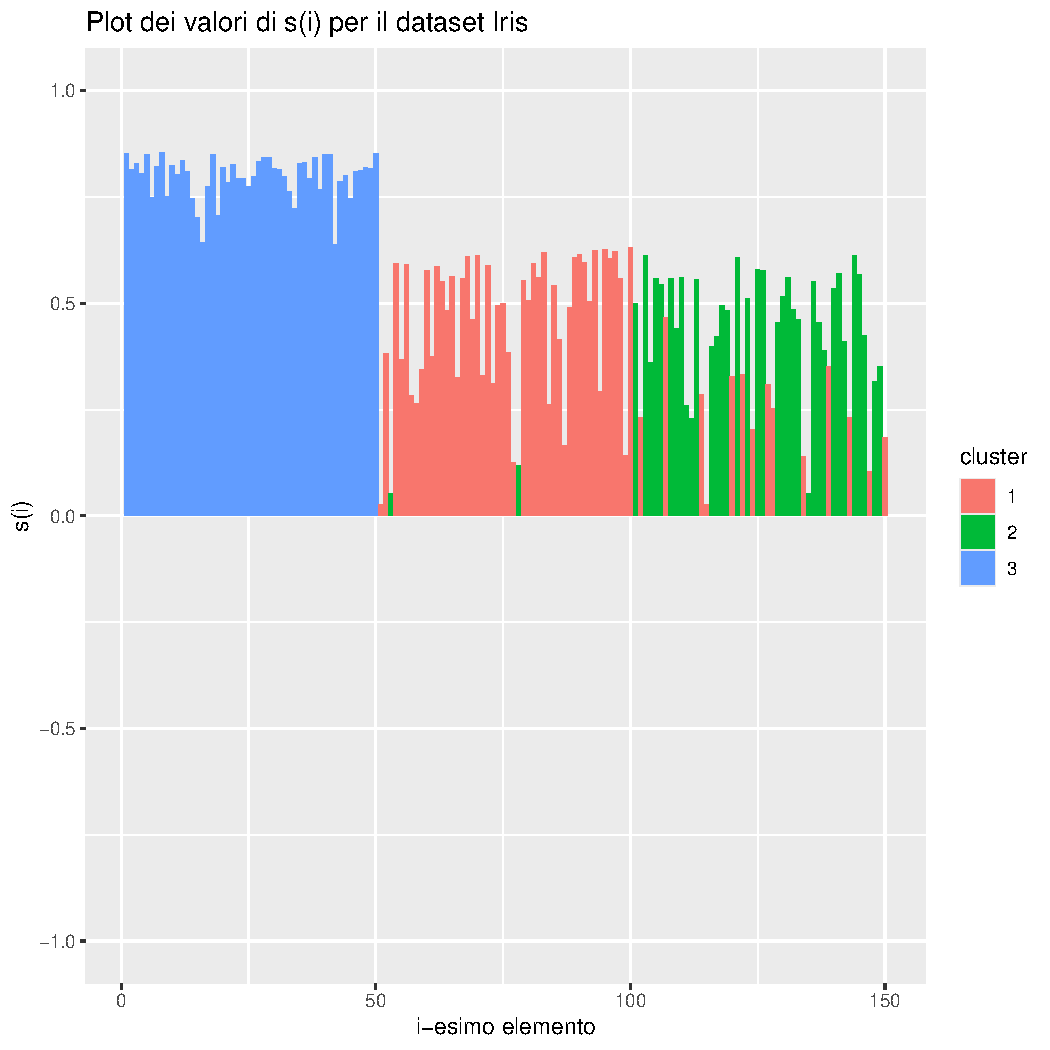
\includegraphics[width = \textwidth]{doc/si.pdf}
				\caption{Silhouette plot per il dataset \texttt{iris}.}
				\label{fig:si}
			\end{figure}

		\section{Come interpretare Silhouette}

			Il vantaggio di Silhouette è che non dipende da quale algoritmo
			è stato usato per effettuare il clustering. Per tale motivo, può
			essere usato per valutare "a posteriori" il risultato dell'algoritmo,
			provando a modificare il valore degli iperparametri per valutare
			quale combinazione di iperparametri restituisce il risultato più
			coerente. Questo riesce particolarmente bene negli algoritmi in
			cui il numero di cluster figura fra gli iperparametri, come K-Means.

			Per esempio, si supponga che un dataset abbia effettivamente
			delle aree molto dense separate da aree ampie vuote. Operando
			un clustering in cui il numero di cluster è più basso del numero
			"naturale" di cluster, delle aree molto distanti tra loro vengono
			inglobate in un cluster unico nonostante vi siano considerevoli
			distanze nel mezzo. Silhouette può evidenziare questa situazione
			perché il valore di $a(i)$ tende ad essere molto alto, essendo
			i membri del dataset molto distanti dai loro centroidi.

			Si supponga invece di operare un clustering in cui il numero
			di cluster è più alto del numero "naturale" di cluster. In tale
			situazione, anche aree dense vengono spezzate in cluster diversi.
			Silhouette può evidenziare questa situazione perché il valore di
			$b(i)$ tende ad essere molto basso, dato che elementi molto vicini
			vengono separati forzosamente.

			\begin{figure}[h]
				\centering
				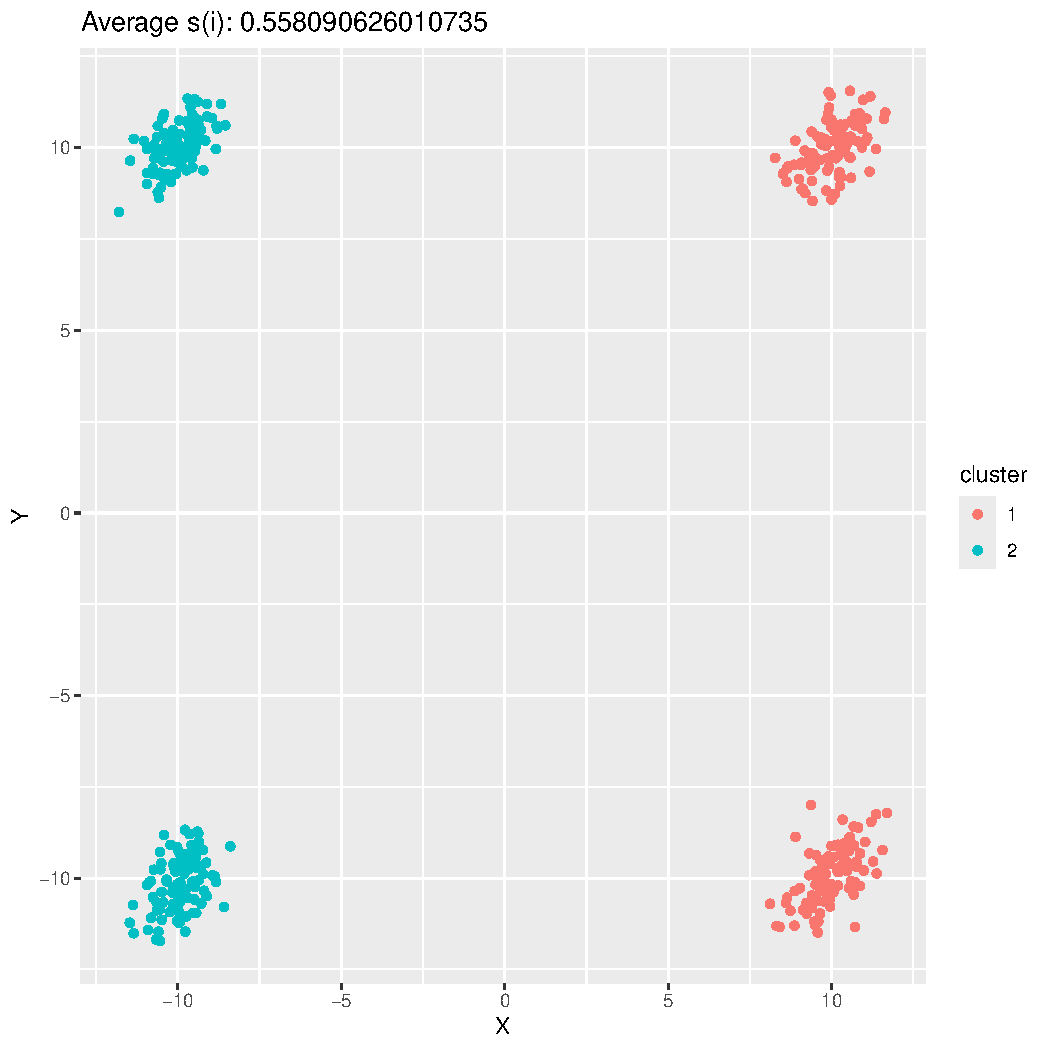
\includegraphics[width = 0.5\textwidth, height = 0.3\textheight]{doc/clusters-2.pdf}
				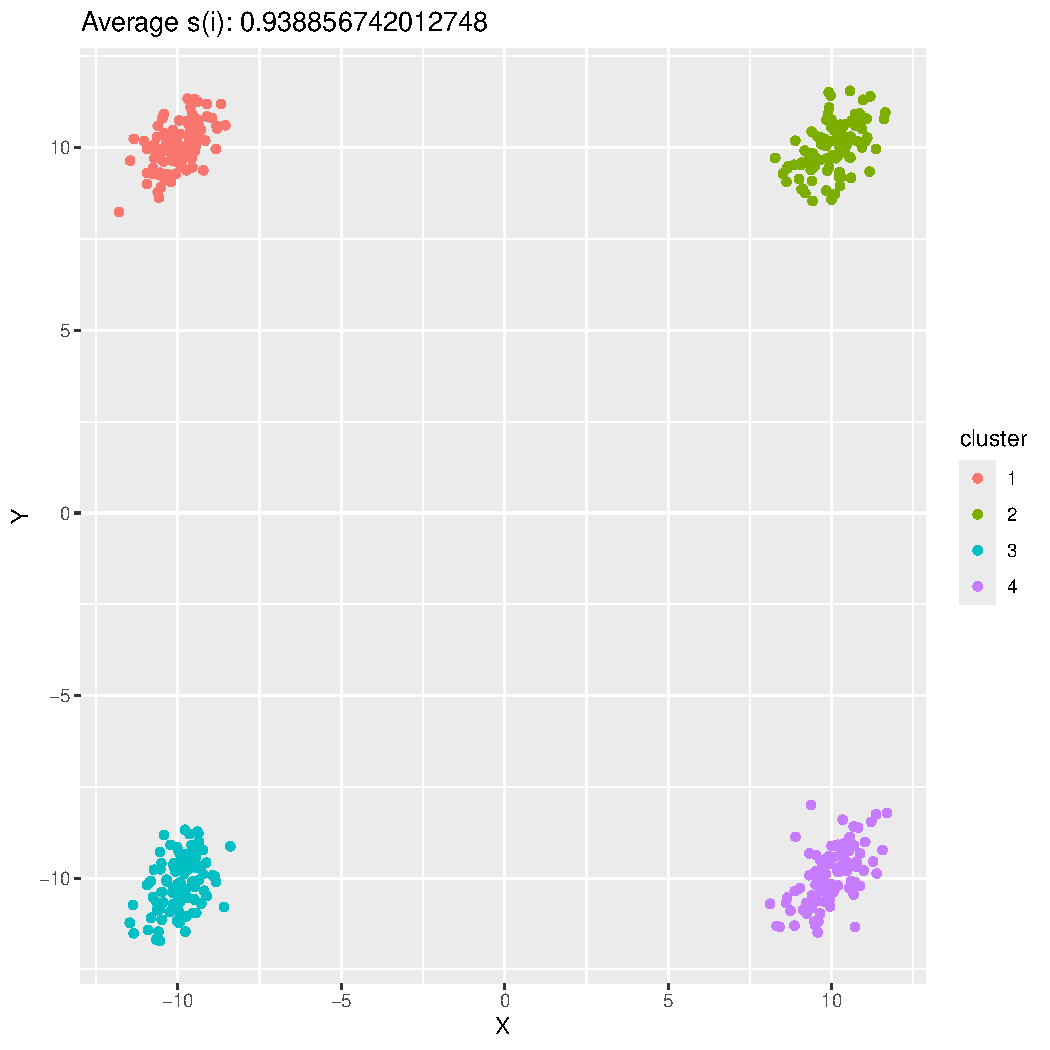
\includegraphics[width = 0.5\textwidth, height = 0.3\textheight]{doc/clusters-4.pdf}
				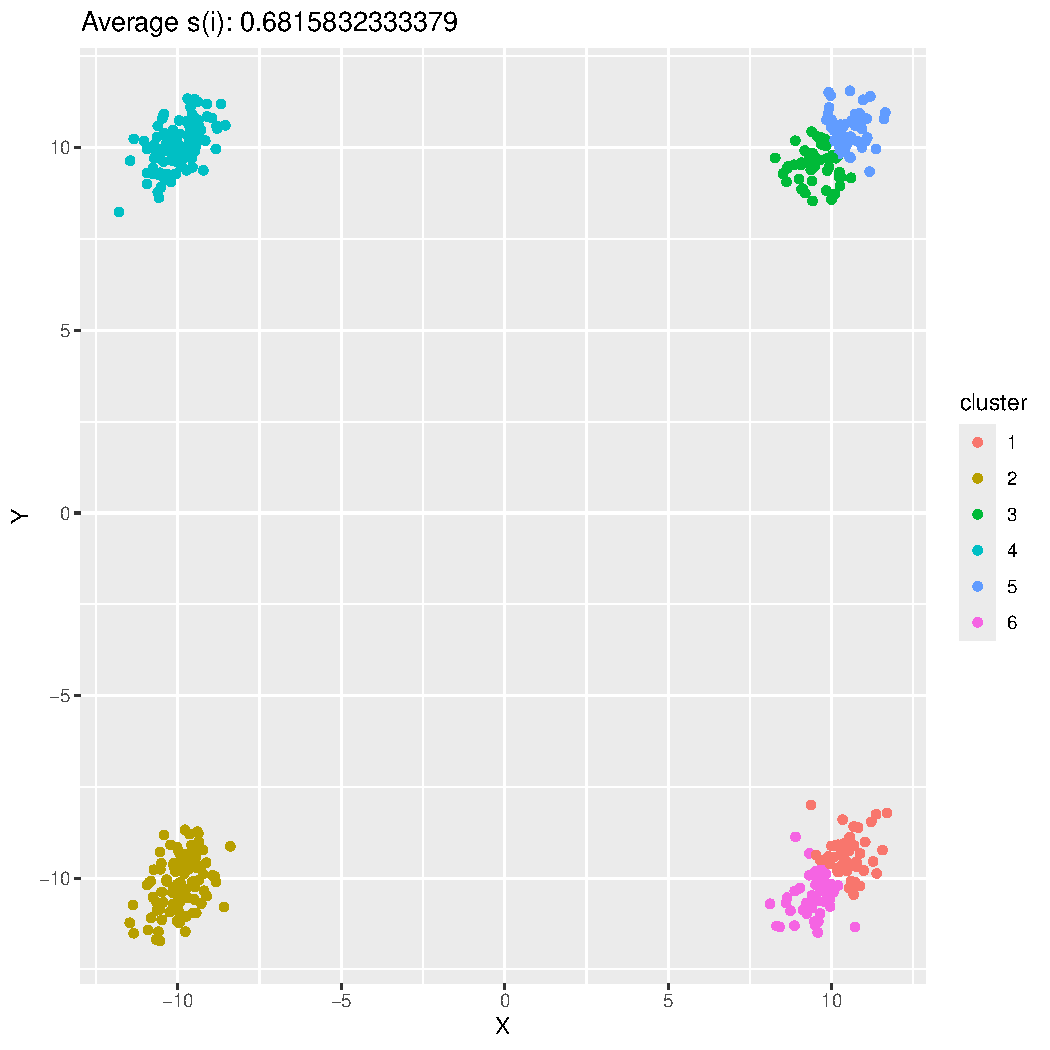
\includegraphics[width = 0.5\textwidth, height = 0.3\textheight]{doc/clusters-6.pdf}
				\caption{Clustering con K-Means usando K = 2, 4, 6 per un dataset
				auto generato in cui la struttura di cluster è ben visibile. }
				\label{fig:k246}
			\end{figure}

			In generale, l'operato di un algoritmo di clustering può
			considerarsi ottimale se il valore si $s(i)$ tende ad essere
			molto alto per tutti gli elementi del dataset. A tale scopo,
			è possibile calcolare la Silhouette media per un certo cluster
			$C$ come la media tutti gli $s(i)$ per ciascun elemento $i$
			che appartiene a $C$. Se tale valore medio è alto, il cluster
			nel suo complesso è ben formato.

			Se si ha invece interesse a sapere qual'è il numero ottimale di
			cluster, è possibile considerare la Silhouette media complessiva
			come la media di tutti gli $s(i)$ per ogni elemento dell'intero
			dataset. L'idea è quella di testare diverse combinazioni di
			iperparametri dell'algoritmo di clustering e scegliere la
			combinazione che restituisce la Silhouette media complessiva più
			grande: tale combinazione sarà quella che restituisce il clustering
			che meglio interpreta il dataset.


			Si noti come un valore della Silhouette media complessiva
			pari a $0$ non significa necessariamente che il clustering
			non sia andato a buon fine. Può infatti anche indicare che
			effettivamente il dataset non ha alcuna struttura di clustering
			naturale, e che quindi l'algoritmo di clustering ha comunque
			fornito un risultato corretto, dato che effettivamente qualsiasi
			risultato vale l'altro.

		\section{Sviluppi futuri}

			A partire dall'idea di base di Silhouette, è possibile costruirne
			infinite varianti. Gli autori citano:

			\begin{itemize}
				\item
				Per determinare il miglior numero di cluster non è strettamente
				necessario utilizzare la Silhouette media complessiva. Sarebbe
				infatti possibile anche combinare gli $s(i)$ in modo diverso;
				\item
				La Silhouette media complessiva può essere essa stessa usata
				come funzione obiettivo da massimizzare direttamente all'interno
				di un algoritmo di clustering, anziché effettuare una valutazione
				a posteriori;
				\item
				Se l'algoritmo di clustering si basa sulla costruzione di centroidi
				o sulla elezione di rappresentanti, si potrebbe usare la distanza
				da tali centroidi o rappresentanti come grado di dissomiglianza
				anziché calcolare $a(i)$ o $D(i, C)$ per ogni $i$-esimo elemento,
				semplificando il procedimento. Naturalmente, questo approccio
				renderebbe Silhouette dipendente dal tipo di algoritmo usato. 
			\end{itemize}

			Tutte e tre le varianti sono toccate da articoli citati.

	\chapter{Scelta dei pacchetti}

		Il linguaggio \texttt{R} offre diverse implementazioni del
		calcolo della Silhouette. Ho cercato alcune fra queste utilizzando
		il sito \texttt{https://rdrr.io} e scegliendone quante più possibili
		che provenissero dal repository CRAN. In particolare, sono stati
		scelti \texttt{cluster}, \texttt{drclust}, \texttt{tidyclust} e
		\texttt{Kira}. Pacchetti noti come \texttt{fpc}, che pure
		implementano Silhouette, li ho esclusi a priori perché non
		aggiornati da tempo.

		Oltre a questi, come controprova ho utilizzato l'implementazione
		della Silhouette presente nel pacchetto \texttt{scikit-learn} per
		\texttt{Python}. Questo è stato fatto attraverso il pacchetto
		\texttt{reticulate}, che permette di chiamare funzioni \texttt{Python}
		all'interno di codice \texttt{R}.

		Per comparare le performance delle diverse implementazioni di
		Silhouette ho eseguito due test, uno chiamato "sanity check" ed
		uno chiamato "matrice binaria". Il codice per la generazione dei
		test è liberamente disponibile. Ho organizzato il codice seguendo
		le linee guida riportate in \cite{10.1371/journal.pcbi.1000424}.
		Ho anche tenuto un lab notebook per tenere traccia dei risultati
		mano mano che venivano generati, facendo riferimento a \cite{10.1371/journal.pcbi.1004385}

		\section{Sanity check}

			Il test Sanity check prevede di utilizzare due dataset creati
			artificialmente, il primo dove la struttura di cluster è
			estremamente evidente ed il secondo dove la struttura di
			cluster è completamente assente, applicare su questi l'algoritmo
			di clustering K-Means e calcolare sul risultato di quest'ultimo
			la Silhouette media.

			Lo scatter plot dei due dataset è riportato in Figure~\ref{fig:sc}.
			Li ho costruiti utilizzando la funzione \texttt{rnorm}, che genera
			dei punti casuali a partire da una distribuzione normale bivariata.
			
			Il primo dataset è stato costruito usando due distribuzioni
			normali fuse insieme, entrambe con una deviazione standard
			molto bassa, di modo che i punti siano concentrati attorno
			alla media. Il secondo dataset è costituito da una sola distribuzione
			normale centrata in $(0, 0)$ con una deviazione standard molto ampia,
			di modo che i punti siano molto dispersi.

			\begin{figure}[h]
				\centering
				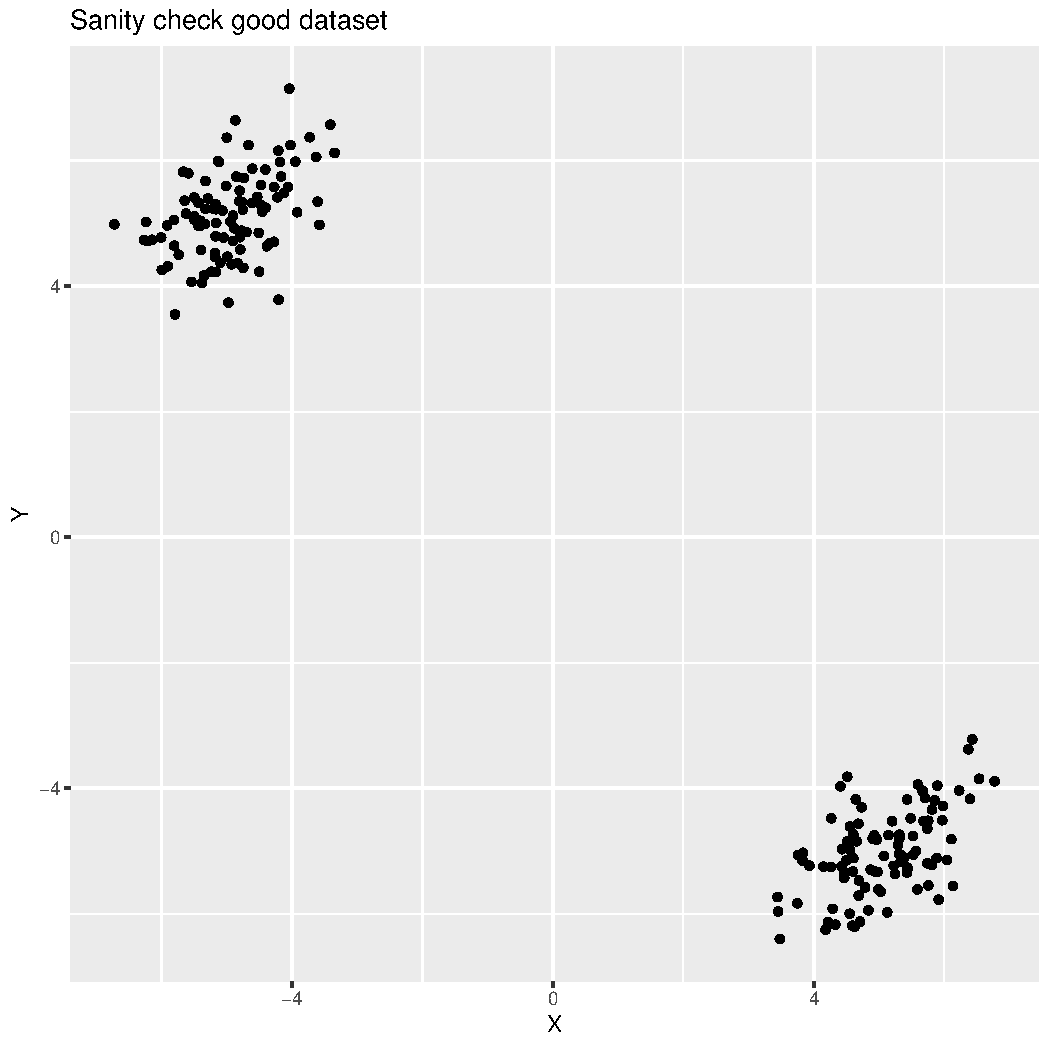
\includegraphics[width = 0.75\textwidth, height = 0.45\textheight]{doc/sc_dataset_good.pdf}
				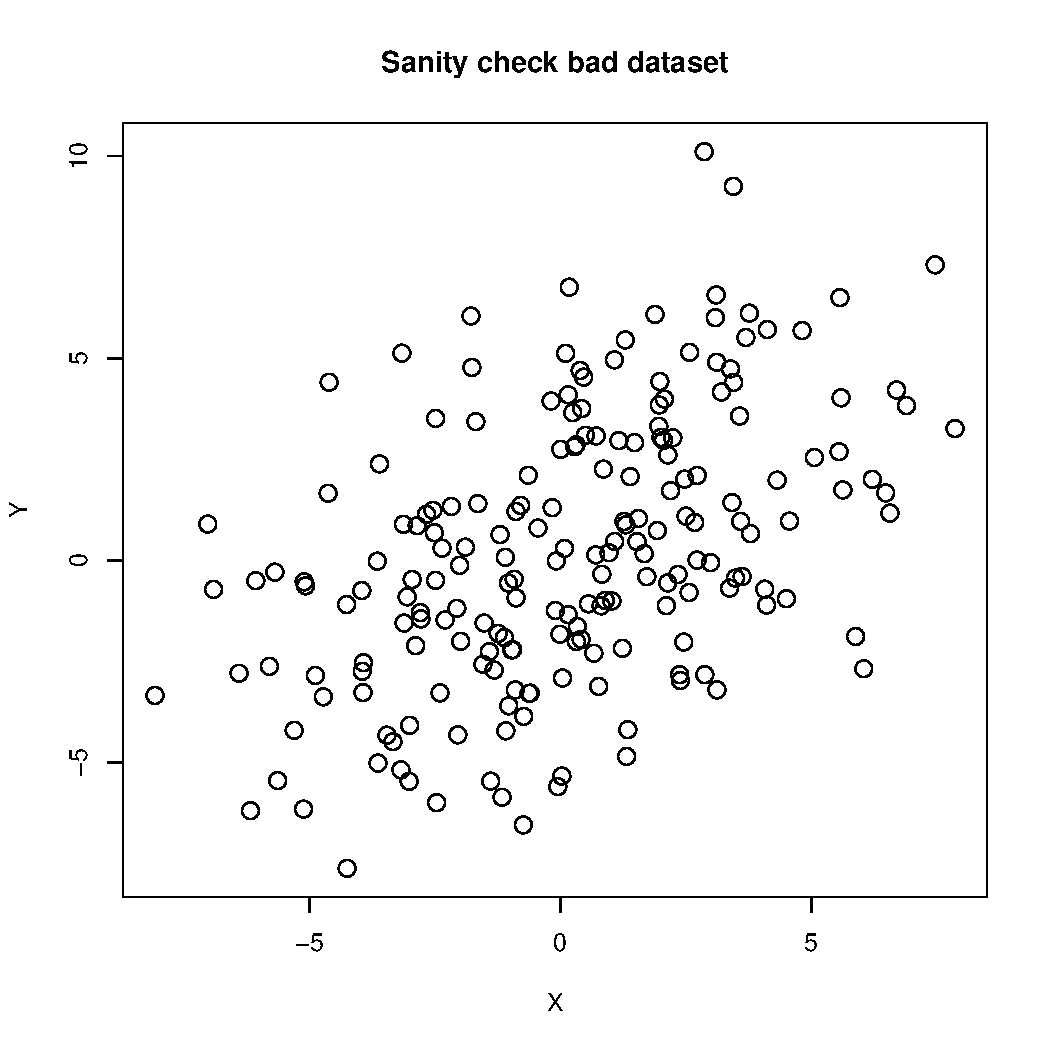
\includegraphics[width = 0.75\textwidth, height = 0.45\textheight]{doc/sc_dataset_bad.pdf}
				\caption{Plot dei dataset per il test sanity check. Il primo
				presenta una struttura di cluster ben definita, mentre nel
				secondo la struttura di cluster è completamente assente.}
				\label{fig:sc}
			\end{figure}

			I risultati per il test sanity check sono riportati di seguito.
			Il test sanity check non é stato particolarmente conclusivo,
			perché tutti e cinque i pacchetti hanno fornito valori molto
			simili (circa $0.9$ per il primo dataset e circa $0.4$ per il
			secondo). Questo é un risultato atteso, perché il test era
			appositamente costruito per escludere pacchetti problematici.

			\begin{figure}[h]
				\begin{boxedminipage}{0.5\textwidth}
					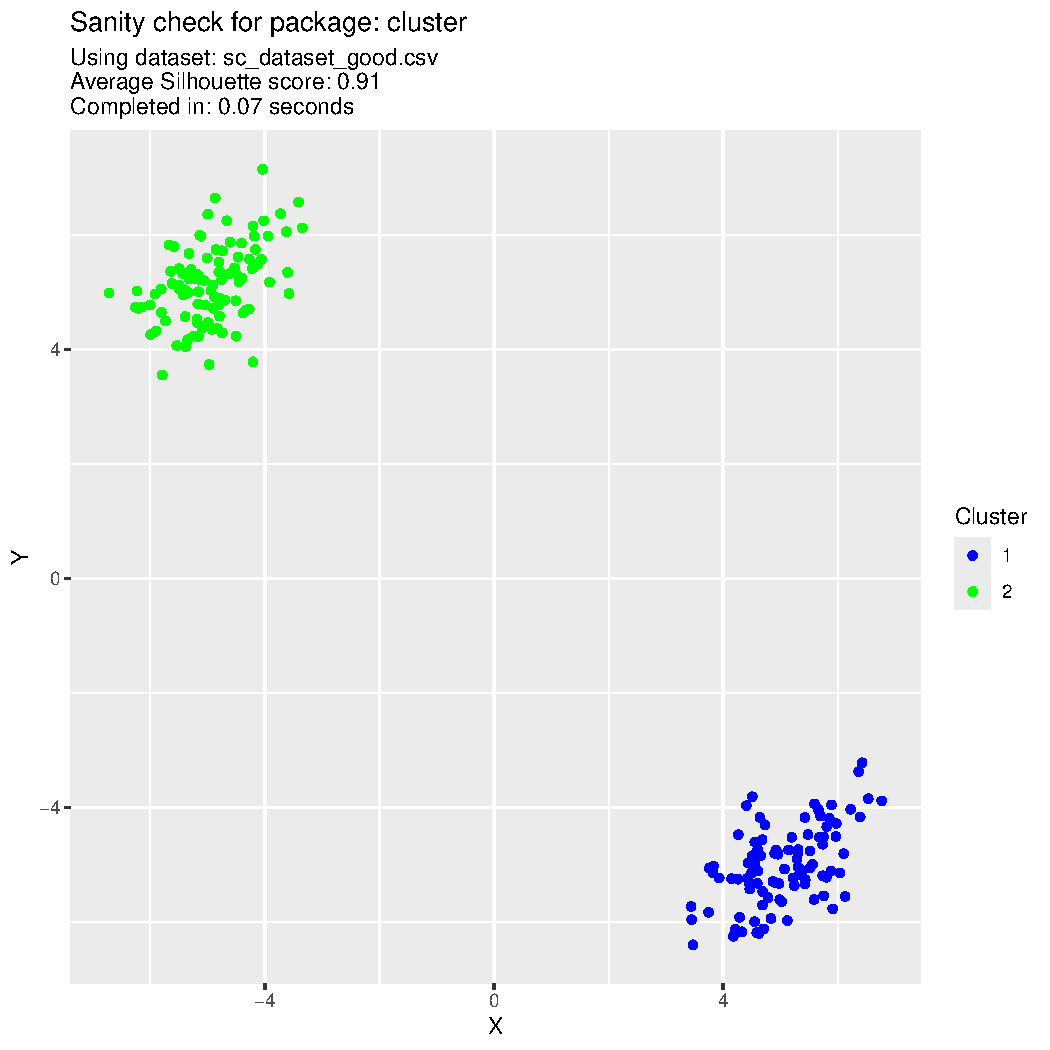
\includegraphics[width = \textwidth, page = 1]{results/results_CLUSTER.pdf}
				\end{boxedminipage}
				\begin{boxedminipage}{0.5\textwidth}
					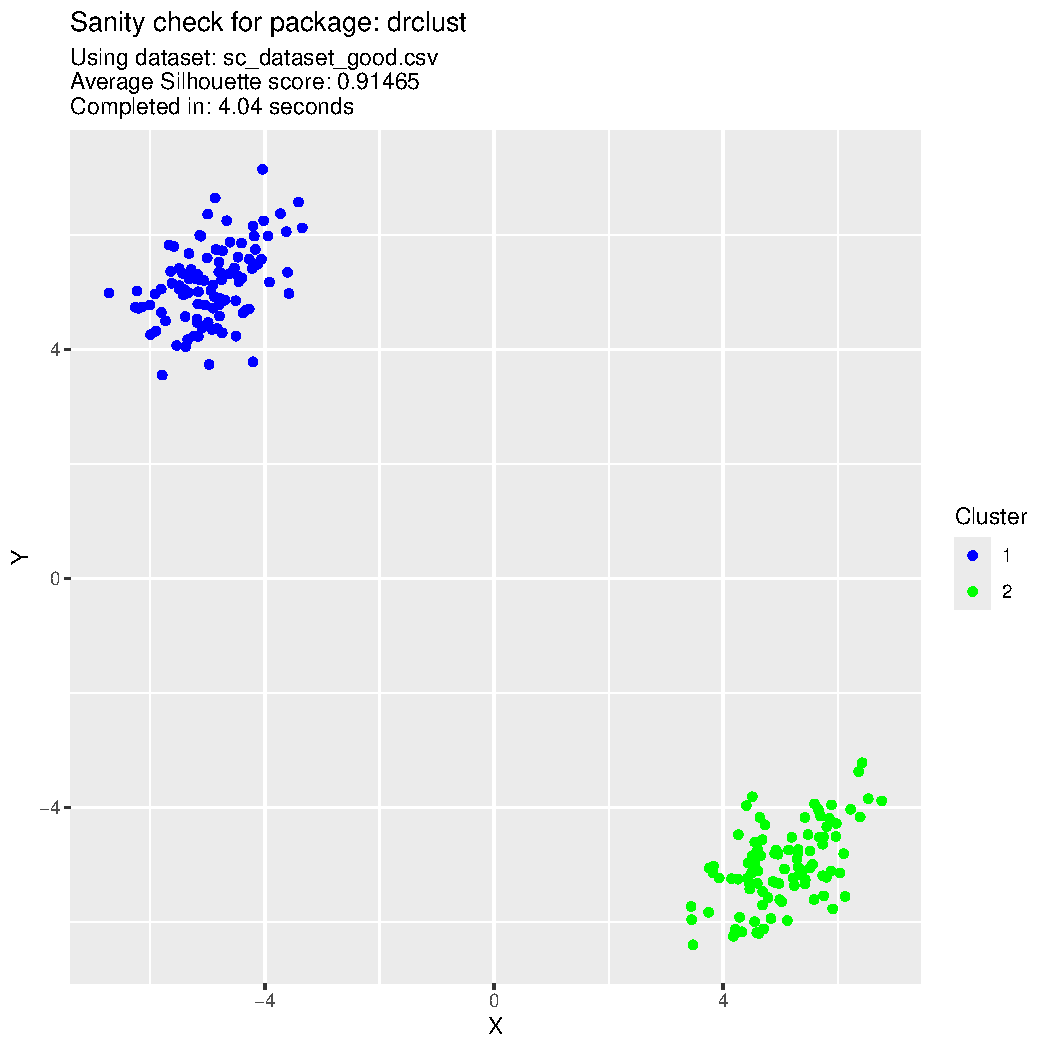
\includegraphics[width = \textwidth, page = 1]{results/results_DRCLUST.pdf}
				\end{boxedminipage}
				\begin{boxedminipage}{0.5\textwidth}
					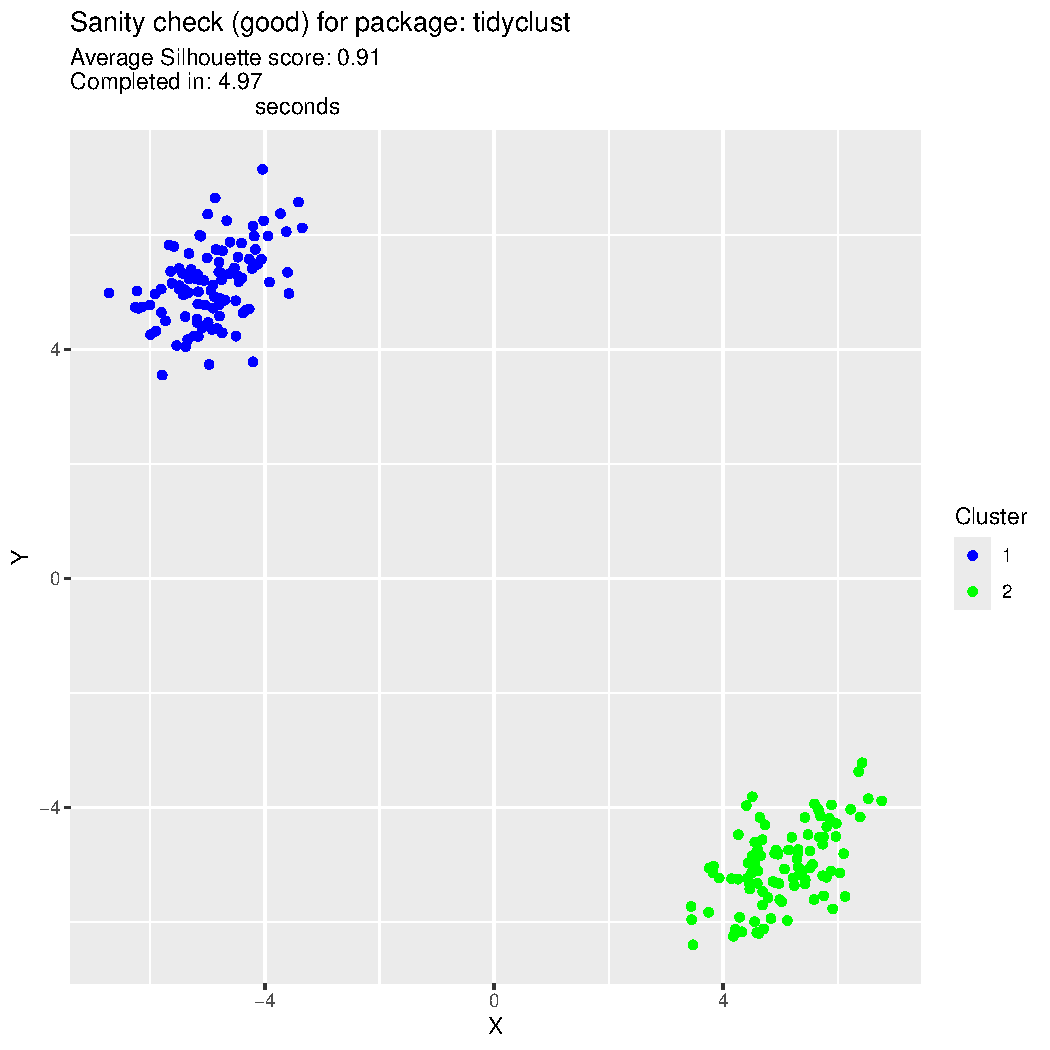
\includegraphics[width = \textwidth, page = 1]{results/results_TIDYCLUST.pdf}
				\end{boxedminipage}
				\begin{boxedminipage}{0.5\textwidth}
					%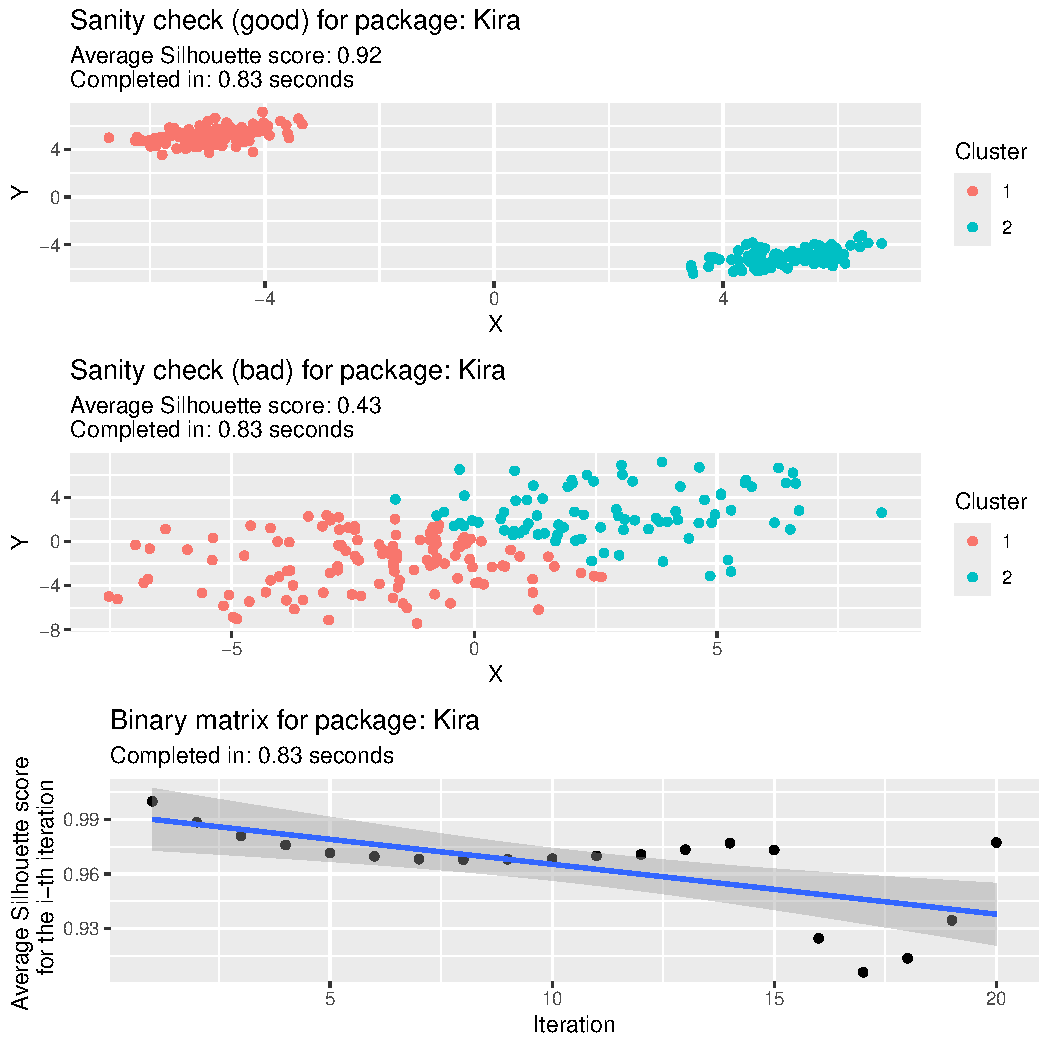
\includegraphics[width = \textwidth, page = 1]{results/results_KIRA.pdf}
				\end{boxedminipage}
				\caption{Plot dei test sanity check usando il dataset con struttura di cluster
				ben visibile.}
				\label{fig:good}
			\end{figure}

			\begin{figure}[h]
				\begin{boxedminipage}{0.5\textwidth}
					\includegraphics[width = \textwidth, page = 2]{results/results_CLUSTER.pdf}
				\end{boxedminipage}
				\begin{boxedminipage}{0.5\textwidth}
					\includegraphics[width = \textwidth, page = 2]{results/results_DRCLUST.pdf}
				\end{boxedminipage}
				\begin{boxedminipage}{0.5\textwidth}
					\includegraphics[width = \textwidth, page = 2]{results/results_TIDYCLUST.pdf}
				\end{boxedminipage}
				\begin{boxedminipage}{0.5\textwidth}
					%\includegraphics[width = \textwidth, page = 2]{results/results_KIRA.pdf}
				\end{boxedminipage}
				\caption{Plot dei test sanity check usando il dataset con struttura di cluster
				assente.}
				\label{fig:bad}
			\end{figure}

			\begin{figure}[h]
				\centering
				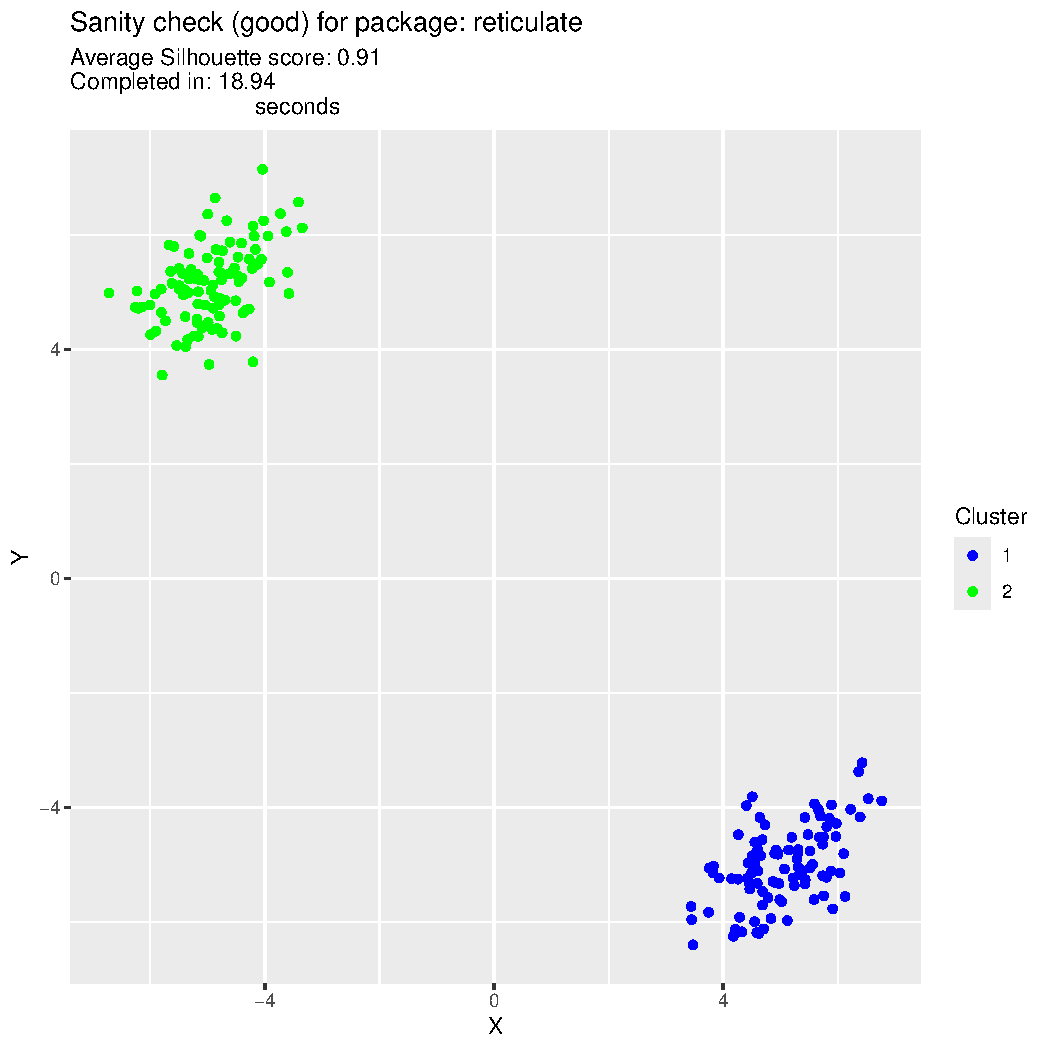
\includegraphics[width = 0.75\textwidth, height = 0.45\textheight, page = 1]{results/results_RETICULATE.pdf}
				\includegraphics[width = 0.75\textwidth, height = 0.45\textheight, page = 2]{results/results_RETICULATE.pdf}
				\caption{Plot del test sanity check usando \texttt{scikit-learn} attraverso
				\texttt{reticulate}.}
				\label{fig:reticulate}
			\end{figure}

		\section{Matrice binaria}

			Il test matrice binaria inizia con una matrice di dimensione
			$2n times n$, costituita per metà da $0$ e per metà da $1$.
			Su tale matrice viene applicato K-Means con iperparametro
			$K = 2$ e si calcola la Silhouette media complessiva del
			risultato. Dopodiché, una qualsiasi delle righe viene sostituita
			con un valore scelto casualmente nell'intervallo $(0, 1)$ e si
			ripete il procedimento. Tale test viene ripetuto esattamente
			$2n$ volte, ogni volta con una riga diversa.

			I $2n$ valori della Silhouette media complessiva così trovati
			sono poi riportati in un plot; l'idea è che tali valori debbano
			essere alti nelle prime istanze del test quando gli $0$ e gli
			$1$ sono ben separati e piano piano perdano si riducano così
			come il dataset perde coesione. Ci si aspetta che i punti sul
			grafico approssimino una distribuzione lineare.

			I risultati per il test matrice binaria sono riportati
			di seguito. Il test é stato piú informativo del precedente,
			perché i valori restituiti avevano delle differenze
			evidenziabili. In particolare, \texttt{Kira} é stato il
			pacchetto con le performance peggiori, perché i valori
			della Silhouette media complessiva sono rimasti pressoché
			identici. I pacchetti \texttt{cluster}, \texttt{drclust}
			e \texttt{tidyclust} hanno invece avuto risultati molto
			simili. In particolare, \texttt{cluster} e \texttt{tidyclust}
			hanno avuto risultati perfettamente identici, segno che
			probabilmente l'uno usa l'altro come subroutine.

			\begin{figure}[h]
				\begin{boxedminipage}{0.5\textwidth}
					\includegraphics[width = \textwidth, page = 3]{results/results_CLUSTER.pdf}
				\end{boxedminipage}
				\begin{boxedminipage}{0.5\textwidth}
					\includegraphics[width = \textwidth, page = 3]{results/results_DRCLUST.pdf}
				\end{boxedminipage}
				\begin{boxedminipage}{0.5\textwidth}
					\includegraphics[width = \textwidth, page = 3]{results/results_TIDYCLUST.pdf}
				\end{boxedminipage}
				\begin{boxedminipage}{0.5\textwidth}
					%\includegraphics[width = \textwidth, page = 3]{results/results_KIRA.pdf}
				\end{boxedminipage}
				\caption{Plot dei test matrice binaria.}
				\label{fig:bm}
			\end{figure}

			\begin{figure}[h]
				\includegraphics[width = \textwidth, page = 3]{results/results_RETICULATE.pdf}
				\caption{Plot del test matrice binaria per il pacchetto
				\texttt{scikit-learn} (attraverso \texttt{reticulate})}
				\label{fig:reticulatebm}
			\end{figure}

		\section{Considerazioni}

			Alla luce dei due test considerati, il pacchetto \texttt{Kira}
			é stato immediatamente escluso, perché i risultati forniti dal
			test della matrice binaria non sono affatto incoraggianti.
			Dato che i pacchetti \texttt{cluster} e \texttt{tidyclust}
			hanno fornito un risultato identico, fra i due é stato preferito
			\texttt{cluster}, perché fra i due era quello con il tempo di
			esecuzione piú basso. Il pacchetto \texttt{scikit-learn}
			attraverso \texttt{reticulate} non é stato preso in
			considerazione, perché era stato incluso semplicemente
			come metro di paragone.

			Fra \texttt{cluster} e \texttt{drclust} ho preferito scegliere
			\texttt{cluster}. Questo sia perché il tempo di esecuzione é
			inferiore, sia perché il pacchetto \texttt{cluster} si trova
			spesso giá incluso nelle installazioni di \texttt{R} (garanzia
			di affidabilitá) sia perché é l'unico pacchetto il cui input
			non dipende dall'algoritmo usato. Infatti, \texttt{cluster}
			ha in input il risultato di un qualsiasi algoritmo di clustering
			ed una matrice delle distanze, mentre gli altri pacchetti
			richiedono in input espressamente il risultato dell'applicazione
			di una loro implementazione di un algoritmo.

			In Figure~\ref{fig:cmp} è presentata la differenza fra
			\texttt{cluster} e \texttt{scikit-learn} sul test matrice
			binaria. Come è possibile notare, la differenza fra i due
			è contenuta.

			\begin{figure}[h]
				\centering
				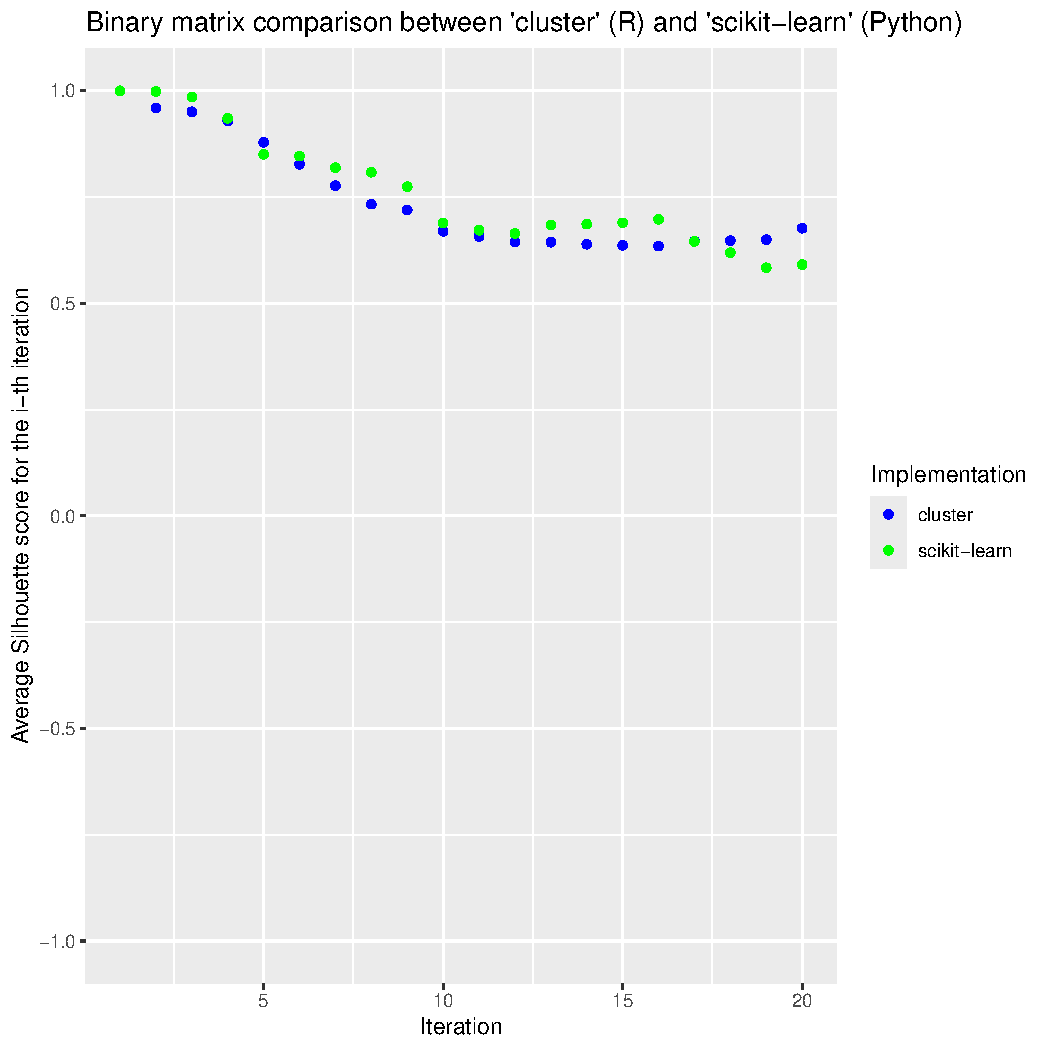
\includegraphics[width = 0.5\textwidth, height = 0.3\textheight, page = 1]{results/Final_comparison.pdf}
				\includegraphics[width = 0.5\textwidth, height = 0.3\textheight, page = 2]{results/Final_comparison.pdf}
				\includegraphics[width = 0.5\textwidth, height = 0.3\textheight, page = 3]{results/Final_comparison.pdf}
				\caption{Differenze fra il test matrice binaria tra \texttt{cluster} (pacchetto R)
				e \texttt{scikit-learn} (pacchetto Python).}
				\label{fig:cmp}
			\end{figure}

	\chapter{Uso di Silhouette su EHR}

		Articoli citati: \cite{Chang2024}, \cite{Alexander2021}, \cite{HYUN2020105507},
		\cite{Josephson_Gonzalez-Izquierdo_Engbers_Denaxas_Delgado-Garcia_Sajobi_Wang_Keezer_Wiebe_2023/10/01_2023},
		\cite{01277230-202011000-00006}.

		\begin{table}[h]
			\centering
			\footnotesize
			\begin{tabular}{| p{1.75cm} | p{1.75cm} | p{1.75cm} | p{1.75cm} | p{1.75cm} | p{1.75cm} |}
				\hline
				\multicolumn{6}{| p{12.5cm} |}{
					\textit{Identifying heterogeneous subgroups of systemic autoimmune
					diseases by applying a joint dimension reduction and clustering
					approach to immunomarkers}
				} \\
				\hline
				\textbf{Patologie} &
				\textbf{N. pazienti} &
				\textbf{Features} &
				\textbf{Algoritmi} &
				\textbf{Software} &
				\textbf{Metriche} \\
				\hline
				Lupus Eritematoso Sistemico, Artrite Reumatoide,
				Sindrome di Sjogren &
				11923 &
				biomarcatori (tradotti in variabili categoriali) &
				Multiple Correspondence Analysis K-means (clustering e dimensionality
				reduction insieme) &
				clustrd (R) &
				Silhouette \\
				\hline
				\multicolumn{6}{| p{12.5cm} |}{
					\textit{Association of comorbid-socioeconomic clusters with
					mortality in late onset epilepsy derived through unsupervised
					machine learning}
				} \\
				\hline
				\textbf{Patologie} &
				\textbf{N. pazienti} &
				\textbf{Features} &
				\textbf{Algoritmi} &
				\textbf{Software} &
				\textbf{Metriche} \\
				\hline
				Epilessia (tardiva) &
				11307 &
				Fattori di rischio, comorbiditá (indice di Charlson) &
				Agglomerative Hierarchical Clustering &
				scikit-learn (Python), Python 3.6.3, Stata 16.1 &
				Silhouette, Davies-Bouldin \\
				\hline
				\multicolumn{6}{| p{12.5cm} |}{
					\textit{Exploration of critical care data by using unsupervised
					machine learning}
				} \\
				\hline
				\textbf{Patologie} &
				\textbf{N. pazienti} &
				\textbf{Features} &
				\textbf{Algoritmi} &
				\textbf{Software} &
				\textbf{Metriche} \\
				\hline
				&
				1503 &
				Valori di test di routine di laboratorio (BUN, creatinina, glucosio, ...) &
				Kmeans &
				R 3.5.2 &
				Total within-cluster variation, Silhouette, Gap statistic \\
				\hline
				\multicolumn{6}{| p{12.5cm} |}{
					\textit{Identifying and evaluating clinical subtypes of Alzheimer’s
					disease in care electronic health records using unsupervised machine
					learning}
				} \\
				\hline
				\textbf{Patologie} &
				\textbf{N. pazienti} &
				\textbf{Features} &
				\textbf{Algoritmi} &
				\textbf{Software} &
				\textbf{Metriche} \\
				\hline
				Malattia di Alzheimer &
				10065 &
				sintomi tipici, comorbiditá, dati demografici &
				K-Means, Kernel K-means, Affinity Propagation, Latent Class Analysis &
				&
				Silhouette, Coefficiente di Jaccard \\
				\hline
				\multicolumn{6}{| p{12.5cm} |}{
					\textit{Utilization of Deep Learning for Subphenotype Identification
					in Sepsis-Associated Acute Kidney Injury}
				} \\
				\hline
				\textbf{Patologie} &
				\textbf{N. pazienti} &
				\textbf{Features} &
				\textbf{Algoritmi} &
				\textbf{Software} &
				\textbf{Metriche} \\
				\hline
				Sepsi &
				4001 &
				Segni vitali, test di laboratorio &
				K-Means &
				scikit-learn (Python), matplotlib (Python), SAS 9.4, R 3.4.3 &
				Silhouette, Davies-Bouldin, Calinksi-Harabasz \\
				\hline
			\end{tabular}
		\end{table}

	\chapter{Aspetti teorici di Silhouette}

		Articoli citati: \cite{10.1007/978-3-030-52348-0_2},
		\cite{doi:10.3233/IDA-2012-0545}, \cite{Gao2019CUBOSAI},
		\cite{NAGHIZADEH2020205}, \cite{10.1007/978-3-319-19369-4_5}.

	\chapter{Dataset reali}

	\printbibliography

\end{document}
